%% Supplementary Information for
%% "Beyond Arbitrariness: Detecting Geographic Structure -- and the Limits of
%%  Current Linguistic Databases"
%%
%% Target journal: Language Sciences (Elsevier).
%% Build: latexmk -pdf supplement.tex   (see scripts/compile_supplement.sh)
%% All tables and figures are generated from Result CSV files by the scripts in
%% supplement/scripts/. This file is an audit/reproducibility layer only; it
%% introduces no new estimates, models, or interpretations.
\documentclass[preprint,12pt]{elsarticle}

\usepackage{lmodern}
\usepackage[T1]{fontenc}
\usepackage[utf8]{inputenc}
\usepackage{booktabs}
\usepackage{graphicx}
\usepackage{amsmath,amssymb}
\usepackage{array}
\usepackage{longtable}
\usepackage{url}
\usepackage{microtype}
\setlength{\emergencystretch}{2em}
\sloppy

% number SI tables/figures as S1, S2, ...
\renewcommand{\thetable}{S\arabic{table}}
\renewcommand{\thefigure}{S\arabic{figure}}
\renewcommand{\thesection}{S\arabic{section}}

\journal{Language Sciences}

\begin{document}

\begin{frontmatter}
\title{Supplementary Information\\
\emph{Beyond Arbitrariness: Detecting Geographic Structure --- and the Limits of
Current Linguistic Databases}}
\author{Author list omitted for anonymised review}
\begin{abstract}
This Supplementary Information is an audit and reproducibility layer for the main
manuscript. Every publication-facing quantity is traceable from the manuscript to
an SI table or figure, from that table or figure to a Result CSV, and from the CSV
to the exact notebook or Python code that generated it. All numerical values are
derived programmatically from the Result CSV files; no value is transcribed from
the manuscript, notebook display output, or PDF. The reported models are
Beta-Binomial hierarchical regressions; the earlier Binomial fits are retained
only as a superseded sensitivity layer. The expensive H100/GPU posterior models
were \emph{not} rerun to build this SI. Throughout, we distinguish word-final vowel
occurrence (measured directly) from open-syllable structure (a plausible
typological correlate), and treat latitude as a composite geographic coordinate
rather than a causal exposure.
\end{abstract}
\end{frontmatter}

\tableofcontents
\clearpage

% ============================================================
\section{Data provenance and preprocessing}
% ============================================================
The two independently assembled databases have partially overlapping language
coverage. Loan forms are excluded (ASJP \texttt{Loan == "true"}; Lexibank
\texttt{Loan} $\in \{$\texttt{true},\texttt{1}$\}$); languages require valid
coordinates and a family identifier and must meet a minimum of 20 concepts.
Word-initial and word-final vowel occurrence are extracted per form and aggregated
to the language level. Table~\ref{tab:s1} summarises provenance; Table~\ref{tab:s2}
gives the segment and vowel classification rules, taken verbatim from the notebook
code.

\begin{table}[htbp]\centering
\footnotesize
\caption{Database provenance and preprocessing summary.}
\label{tab:s1}
\resizebox{\ifdim\width>\linewidth \linewidth\else\width\fi}{!}{%
\begin{tabular}{p{0.30\textwidth} p{0.32\textwidth} p{0.30\textwidth}}
\toprule
Attribute & ASJP & Lexibank \\
\midrule
Version / commit SHA & ASJP (CLDF), SHA \texttt{012795349540} & Lexibank-analysed, SHA \texttt{edf5f028de7e} \\
Raw forms (pre-exclusion) & not recorded in committed CSVs & not recorded in committed CSVs \\
Retained word tokens & 560,372 & 1,740,092 \\
Pre-filter language summaries & 11,393 & 5,501 \\
Inferential languages & 10,886 & 5,501 \\
Family identifiers (primary) & 646 & 298 \\
Transcription system & ASJPcode (41 symbols) & IPA segments (CLTS) \\
Coordinate source & ASJP \texttt{languages.csv} Lat/Long & Lexibank CLDF Lat/Long \\
Family source & ASJP CLDF classification & Glottolog \texttt{Family} ($\rightarrow$ \texttt{Family\_in\_Data}) \\
\bottomrule
\end{tabular}
}

\par\smallskip{\footnotesize\emph{Note.} Retained word tokens are summed from the family-count CSVs; raw pre-exclusion form totals are not stored in the committed Result CSVs. Family-identifier counts are the primary inferential sample (isolate/unknown languages carry unique identifiers).}
\end{table}

\begin{table}[htbp]\centering
\footnotesize
\caption{Segment and vowel classification rules.}
\label{tab:s2}
\resizebox{\ifdim\width>\linewidth \linewidth\else\width\fi}{!}{%
\begin{tabular}{p{0.20\textwidth} p{0.36\textwidth} p{0.36\textwidth}}
\toprule
Rule & ASJP & Lexibank (IPA) \\
\midrule
Vowel definition & character in ASJP\_VOWELS = \{i e E 3 a u o\} & token whose first non-diacritic character is an IPA vowel (25-symbol set) \\
Ignored / stripped symbols & keep only ASJP vowel/consonant symbols; all modifiers dropped & strip length, nasalisation, phonation, stress, tone diacritics (IPA\_STRIP) before classifying \\
Segment extraction rule & per-character: retain symbols in the ASJP vowel or consonant set & split \texttt{Segments} on spaces (\texttt{+}$\rightarrow$space); drop empty tokens \\
Initial-segment rule & initial vowel $=1$ iff first segment is a vowel & initial vowel $=1$ iff first segment is a vowel \\
Final-segment rule & final vowel $=1$ iff last segment is a vowel; final cluster $=$ trailing consonant count & same rule applied to IPA segments \\
Malformed / empty forms & non-string or no valid segment $\rightarrow$ empty list, language contributes no counts & non-string/empty or all-diacritic $\rightarrow$ dropped \\
\bottomrule
\end{tabular}
}

\par\smallskip{\footnotesize\emph{Note.} Definitions taken verbatim from notebook cell~6 (\texttt{ASJP\_VOWELS}, \texttt{IPA\_VOWELS}, \texttt{IPA\_STRIP}, \texttt{asjp\_segments}, \texttt{ipa\_segments}, \texttt{final\_cluster}) and the aggregation in cell~7. Word-final vowel occurrence is measured directly; it is a plausible correlate of, but not identical to, open-syllable structure.}
\end{table}

\clearpage

% ============================================================
\section{Sample flow and metadata audits}
% ============================================================
Table~\ref{tab:s3} traces the ASJP sample from the full language summary to the
primary inferential sample and the macroarea-linked subset. 507 languages are
removed by the 20-concept inclusion threshold. A further 260 languages could not
be linked under the identifier used for the macroarea table; these are not
missing-macroarea cases --- all 260 are isolate/unknown languages carrying unique
family identifiers. Table~\ref{tab:s4} gives the macroarea composition and
Table~\ref{tab:s5} the linkage audit summary; the complete 260-language ledger is
retained in the repository as \texttt{asjp\_macroarea\_dropped\_languages.csv}.

\begin{table}[htbp]\centering
\footnotesize
\caption{ASJP sample flow.}
\label{tab:s3}
\resizebox{\ifdim\width>\linewidth \linewidth\else\width\fi}{!}{%
\begin{tabular}{p{0.44\textwidth} r r r}
\toprule
Stage & Languages & Family ids & Isolate/unknown \\
\midrule
ASJP language summary before primary filter & 11,393 & 667 & 278 \\
Primary complete-case sample (n\_concepts >= 20) & 10,886 & 646 & 260 \\
Macroarea complete-case sample & 10,626 & 386 & 0 \\
\bottomrule
\end{tabular}
}

\par\smallskip{\footnotesize\emph{Note.} 507 languages were removed by the 20-concept inclusion threshold (11{,}393 $\rightarrow$ 10{,}886). A further 260 languages could not be linked under the identifier used for the macroarea table; these are NOT missing-macroarea cases -- all 260 are isolate/unknown languages with unique family identifiers (full ledger: \texttt{asjp\_macroarea\_dropped\_languages.csv}).}
\end{table}

\begin{table}[htbp]\centering
\footnotesize
\caption{Macroarea-linked sample composition.}
\label{tab:s4}
\resizebox{\ifdim\width>\linewidth \linewidth\else\width\fi}{!}{%
\begin{tabular}{l r r r}
\toprule
Macroarea & Languages & Family ids & Share of matched sample \\
\midrule
Africa & 3,570 & 53 & 33.6\% \\
Papunesia & 2,895 & 126 & 27.2\% \\
Eurasia & 2,655 & 38 & 25.0\% \\
North America & 692 & 72 & 6.5\% \\
South America & 508 & 86 & 4.8\% \\
Australia & 306 & 29 & 2.9\% \\
\textbf{Total} & \textbf{10,626} & 386 & 100.0\% \\
\bottomrule
\end{tabular}
}

\par\smallskip{\footnotesize\emph{Note.} Matched macroarea-complete sample (10{,}626 languages, 386 family identifiers). Shares are of the matched sample; family identifiers are not additive across macroareas.}
\end{table}

\begin{table}[htbp]\centering
\footnotesize
\caption{Macroarea linkage audit summary.}
\label{tab:s5}
\resizebox{\ifdim\width>\linewidth \linewidth\else\width\fi}{!}{%
\begin{tabular}{l r r r}
\toprule
Linkage outcome & Languages & Family ids & Isolate/unknown \\
\midrule
included & 10,626 & 386 & 0 \\
no\_macroarea\_match\_by\_Language\_ID & 260 & 260 & 260 \\
\bottomrule
\end{tabular}
}

\par\smallskip{\footnotesize\emph{Note.} Macroarea source: ASJP \texttt{languages.csv} column \texttt{Macroarea}; inner merge on \texttt{Language\_ID}; 11,540 source rows, 0 duplicate identifiers, 11,115 languages with a macroarea. The complete 260-language exclusion ledger is retained as \texttt{asjp\_macroarea\_dropped\_languages.csv}; every excluded language is isolate/unknown, not a missing-macroarea case.}
\end{table}

\clearpage

% ============================================================
\section{Statistical model specifications}
% ============================================================
The reported models are hierarchical Beta-Binomial regressions of the language-level
count of word-final vowels out of total forms. The linear predictor is
$\eta = \alpha + \beta_{\mathrm{lat}}\,z_{\mathrm{lat}} +
\sigma_{\mathrm{family}}\,z_{\mathrm{family}[i]}$, with a Beta-Binomial observation
model $y \sim \mathrm{BetaBinomial}(n,\ \mu\phi,\ (1-\mu)\phi)$,
$\mu = \mathrm{logit}^{-1}\eta$. Family random intercepts condition on family-level
clustering; they are not full phylogenetic control. The positional model adds
language-level intercepts, and the initial--final contrast is a within-language
comparison. Latitude is the absolute value of the coordinate, z-scored with
population standard deviation; it is a composite geographic coordinate, not a
causal exposure. Priors are read directly from the code (Table~\ref{tab:s6}), not
inferred from posteriors. The full model inventory spans the primary model, the
Lexibank replication, the joint initial--final positional model, the
within/between-family decomposition, the matched-sample family-only and
family-plus-macroarea models, the hemisphere-interaction and Southern-Hemisphere
macroarea-specific models, the leave-family-out and leave-top-two positional
re-fits, and the superseded Binomial sensitivity layer.

\begin{table}[htbp]\centering
\footnotesize
\caption{Prior specification and parameterisation.}
\label{tab:s6}
\resizebox{\ifdim\width>\linewidth \linewidth\else\width\fi}{!}{%
\begin{tabular}{p{0.24\textwidth} p{0.24\textwidth} p{0.44\textwidth}}
\toprule
Parameter & Prior & Role \\
\midrule
$\alpha$ (intercept) & $\mathrm{Normal}(0,\,1.5)$ & global log-odds intercept \\
$\beta_{\mathrm{lat}}$ and all slope terms & $\mathrm{Normal}(0,\,1)$ & latitude / level / interaction slopes (\texttt{beta\_lat}, \texttt{beta\_lat\_north}, \texttt{beta\_south\_level}, \texttt{beta\_lat\_south\_delta}, \texttt{beta\_between}, \texttt{beta\_within}, \texttt{beta\_lat\_initial}, \texttt{beta\_final\_level}, \texttt{beta\_lat\_final\_delta}) \\
$\sigma_{\mathrm{family}},\ \sigma_{\mathrm{language}}$ & $\mathrm{Exponential}(1)$ & random-effect standard deviations (family; and language in the positional model) \\
$z_{\mathrm{family}},\ z_{\mathrm{language}}$ & $\mathrm{Normal}(0,1)$, then mean-centred & non-centred, sum-to-zero standardised random intercepts \\
macroarea effects & $\mathrm{Normal}(0,\,0.75)$ & fixed categorical intercepts/slopes for the six observed macroareas (deliberately NOT hierarchical) \\
$\phi$ (Beta-Binomial concentration) & $\mathrm{LogNormal}(\log 20,\,1)$ & overdispersion parameter of the reported Beta-Binomial likelihood \\
\bottomrule
\end{tabular}
}

\par\smallskip{\footnotesize\emph{Note.} Likelihoods: $y \sim \mathrm{Binomial}(n,\ \mathrm{logit}^{-1}\eta)$ (superseded layer) and $y \sim \mathrm{BetaBinomial}(n,\ \mu\phi,\ (1-\mu)\phi)$ with $\mu=\mathrm{logit}^{-1}\eta$ (reported layer); linear predictor $\eta=\alpha+\beta_{\mathrm{lat}}\,z_{\mathrm{lat}}+\sigma_{\mathrm{family}}z_{\mathrm{family}[i]}$. Latitude is $|\mathrm{Latitude}|$ z-scored with population SD (\texttt{ddof=0}); it is a composite geographic coordinate, not a causal exposure. Family random intercepts model family-level clustering and are NOT full phylogenetic control. The positional model adds language-level intercepts; the initial--final contrast is a within-language comparison. Priors are read from notebook cells 11 and 70, not inferred from posteriors.}
\end{table}

\clearpage

% ============================================================
\section{MCMC sampling diagnostics}
% ============================================================
All reported Beta-Binomial models used NUTS with target acceptance 0.99,
maximum tree depth 12, 2000 warm-up and 2500 post-warm-up draws per chain across
4 chains. Table~\ref{tab:s7} reports convergence for every publication-facing
model; all show $\hat{R} \le 1.01$ and zero divergences.

\begin{table}[htbp]\centering
\footnotesize
\caption{Complete MCMC diagnostics for the reported Beta-Binomial models.}
\label{tab:s7}
\resizebox{\ifdim\width>\linewidth \linewidth\else\width\fi}{!}{%
\begin{tabular}{l l r r c c c c r r c c l}
\toprule
Model & Status & N lang. & N fam. & Chains & Warm-up & Draws/chain & Max $\hat{R}$ & Min bulk ESS & Min tail ESS & Div. & Target & Seed \\
\midrule
Primary (ASJP) & primary & 10,886 & 646 & 4 & 2000 & 2500 & 1.00 & 2,062 & 4,128 & 0 & 0.99 & 20260711+301 \\
Replication (Lexibank) & replication & 5,501 & 298 & 4 & 2000 & 2500 & 1.00 & 2,593 & 4,694 & 0 & 0.99 & 20260711+305 \\
Within/between-family & robustness & 10,886 & 646 & 4 & 2000 & 2500 & 1.00 & 1,357 & 2,504 & 0 & 0.99 & 20260711+302 \\
Initial-vs-final (positional) & robustness & 10,886 & 646 & 4 & 2000 & 2500 & 1.00 & 562 & 990 & 0 & 0.99 & 20260711+303 \\
Hemisphere & robustness & 10,886 & 646 & 4 & 2000 & 2500 & 1.01 & 1,428 & 3,375 & 0 & 0.99 & 20260711+304 \\
Family + macroarea & robustness & 10,626 & 386 & 4 & 2000 & 2500 & 1.00 & 2,992 & 4,630 & 0 & 0.99 & 20260711+306 \\
Matched, no macroarea & robustness & 10,626 & 386 & 4 & 2000 & 2500 & 1.00 & 2,056 & 3,699 & 0 & 0.99 & 20260711+308 \\
Southern macroarea slopes & robustness & 4,075 & -- & 4 & 2000 & 2500 & 1.00 & 2,218 & 4,203 & 0 & 0.99 & 20260711+307 \\
\bottomrule
\end{tabular}
}

\par\smallskip{\footnotesize\emph{Note.} Leave-family-out and leave-top-two positional re-fits use the same NUTS settings (target 0.99, max\_tree\_depth 12, 2000 warm-up, 2500 draws/chain, 4 chains) but their R-hat/ESS were not saved to separate diagnostics CSVs; their point estimates appear in Tables S10--S11. Southern macroarea per-macroarea family counts are in Table S15. All reported models show 0 divergences.}
\end{table}

\clearpage

% ============================================================
\section{Binomial versus Beta-Binomial sensitivity}
% ============================================================
The Binomial fits are retained only as a superseded sensitivity layer.
Table~\ref{tab:s8} pairs the two likelihoods; Figure~\ref{fig:s2} compares their
posterior predictive behaviour on three summary statistics. The Binomial recovers
the overall mean but underestimates between-language dispersion; the Beta-Binomial
substantially improves dispersion. Both still underpredict the exact-one boundary
mass --- the Beta-Binomial does not perfectly fit the full distribution. Because no
per-bin Binomial predictive output was stored, Figure~\ref{fig:s2} compares summary
statistics only and does not reconstruct a distribution from summaries.

\begin{table}[htbp]\centering
\footnotesize
\caption{Binomial versus Beta-Binomial coefficient comparison (ASJP).}
\label{tab:s8}
\resizebox{\ifdim\width>\linewidth \linewidth\else\width\fi}{!}{%
\begin{tabular}{l l l}
\toprule
Quantity & Binomial (superseded) & Beta-Binomial (reported) \\
\midrule
Primary latitude & -0.190 [-0.203, -0.177] & -0.151 [-0.195, -0.105] \\
Initial-position latitude & 0.009 [-0.026, 0.044] & 0.029 [-0.005, 0.063] \\
Final-position latitude & -0.257 [-0.291, -0.222] & -0.285 [-0.316, -0.252] \\
Final-minus-initial & -0.266 [-0.275, -0.256] & -0.313 [-0.342, -0.284] \\
Between-family latitude & -0.512 [-0.648, -0.377] & -0.348 [-0.431, -0.266] \\
Within-family latitude & -0.083 [-0.089, -0.078] & -0.033 [-0.055, -0.011] \\
\bottomrule
\end{tabular}
}

\par\smallskip{\footnotesize\emph{Note.} Posterior median [95\% credible interval]. The Binomial fits are the earlier layer; the Beta-Binomial fits are the reported layer, adopted because the Binomial understated between-language dispersion (Figure S2).}
\end{table}


\begin{figure}[htbp]\centering
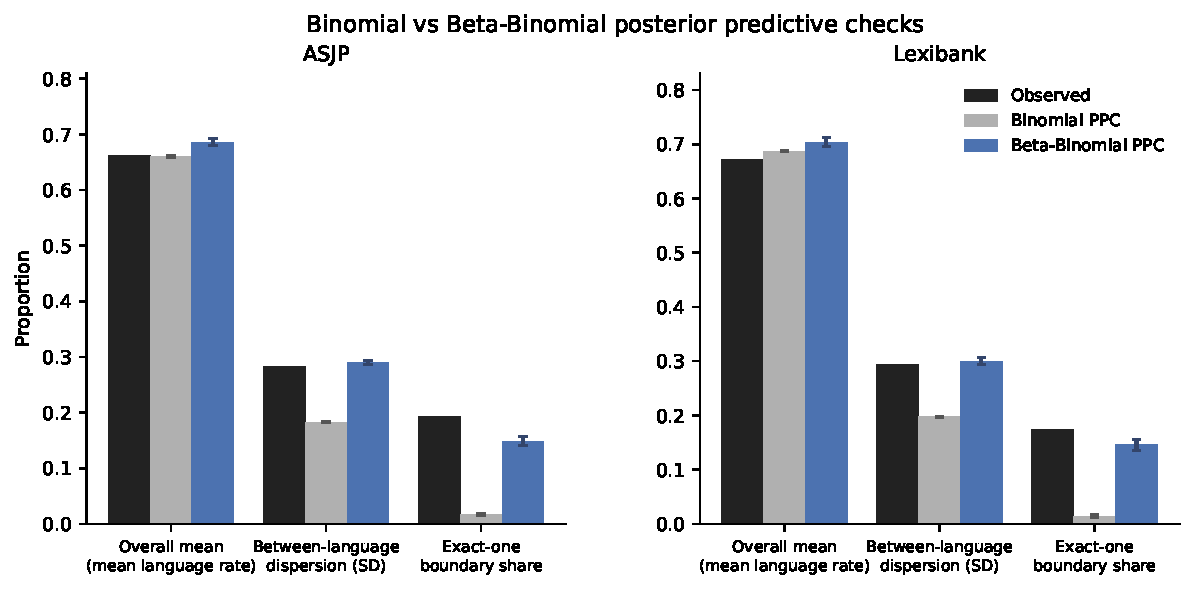
\includegraphics[width=\textwidth]{figures/figureS2_binomial_vs_betabinomial_ppc.pdf}
\caption{Binomial versus Beta-Binomial posterior predictive comparison for ASJP and
Lexibank. Bars show the observed value, the Binomial posterior predictive median,
and the Beta-Binomial posterior predictive median (error bars: 95\% predictive
interval) for the overall mean language rate, the between-language dispersion
(standard deviation), and the exact-one boundary share. The overall mean is
recovered by both likelihoods; the Binomial underestimates dispersion while the
Beta-Binomial recovers it; both underpredict the exact-one boundary share, the
Beta-Binomial less severely. Source: \texttt{figures/figureS2\_source.csv}.}
\label{fig:s2}
\end{figure}
\clearpage

% ============================================================
\section{Lexical-coverage robustness}
% ============================================================
The upper-boundary concentration is not merely a sparse-wordlist artifact. The
robustness sweep in Table~\ref{tab:s9} and Figure~\ref{fig:s3} varies the minimum
\emph{total word count} (not the concept count); the inferential inclusion criterion
throughout the paper is a fixed minimum of 20 concepts. Boundary mass consistent
with boundary inflation or unresolved mixture structure persists across thresholds.
This does not identify a typological class.

\begin{table}[htbp]\centering
\footnotesize
\caption{Boundary mass by minimum total word count.}
\label{tab:s9}
\resizebox{\ifdim\width>\linewidth \linewidth\else\width\fi}{!}{%
\begin{tabular}{l r r r r r r}
\toprule
Database & Min.\ total words & N lang. & Median total words & Share $=1.00$ & Share $\ge 0.99$ & Share $\ge 0.95$ \\
\midrule
ASJP & 20 & 10,886 & 40 & 0.192 & 0.195 & 0.257 \\
ASJP & 40 & 5,655 & 57 & 0.180 & 0.184 & 0.253 \\
ASJP & 60 & 2,699 & 88 & 0.179 & 0.188 & 0.272 \\
ASJP & 80 & 1,850 & 96 & 0.194 & 0.206 & 0.292 \\
ASJP & 100 & 743 & 109 & 0.106 & 0.137 & 0.190 \\
Lexibank & 20 & 5,501 & 214 & 0.173 & 0.237 & 0.323 \\
Lexibank & 40 & 5,501 & 214 & 0.173 & 0.237 & 0.323 \\
Lexibank & 60 & 5,501 & 214 & 0.173 & 0.237 & 0.323 \\
Lexibank & 80 & 5,501 & 214 & 0.173 & 0.237 & 0.323 \\
Lexibank & 100 & 5,009 & 230 & 0.160 & 0.230 & 0.311 \\
\bottomrule
\end{tabular}
}

\par\smallskip{\footnotesize\emph{Note.} The robustness sweep varies the minimum \emph{total word count} (\texttt{min\_n\_total}); it is NOT a concept-count sweep. The inferential inclusion criterion throughout the paper is a fixed minimum of 20 concepts. The committed CSV records median total words, not median concepts. Upper-boundary concentration persists across thresholds, so it is not merely a sparse-wordlist artifact; this does not identify a typological class.}
\end{table}


\begin{figure}[htbp]\centering
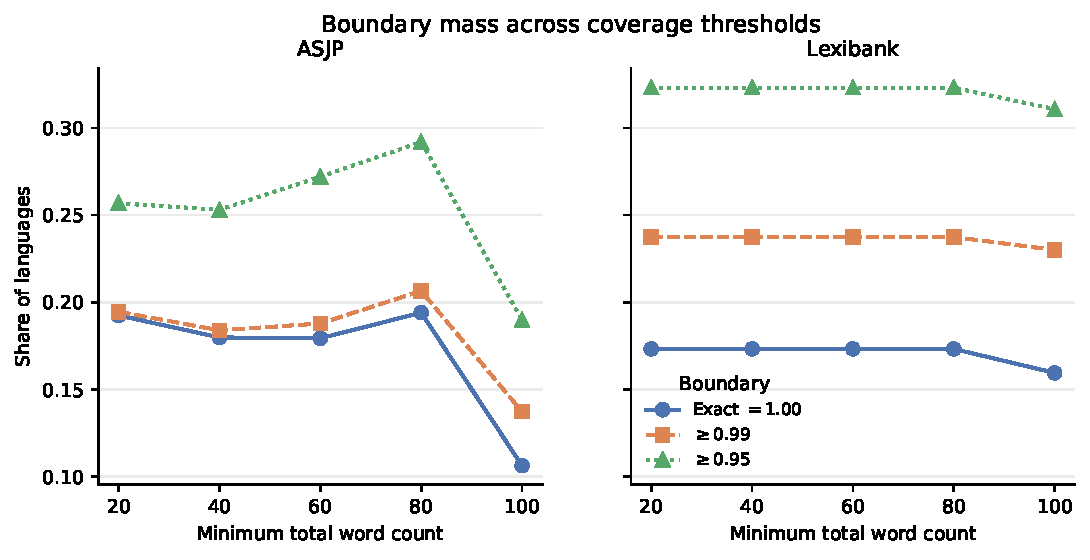
\includegraphics[width=\textwidth]{figures/figureS3_boundary_mass_coverage.pdf}
\caption{Boundary mass across coverage thresholds for ASJP and Lexibank. Each panel
plots the share of languages with word-final vowel rate exactly $1.00$, at least
$0.99$, and at least $0.95$, against the minimum total word count. The inferential
inclusion criterion is a fixed minimum of 20 concepts; this figure varies only the
minimum total word count. Source: \texttt{figures/figureS3\_source.csv}.}
\label{fig:s3}
\end{figure}
\clearpage

% ============================================================
\section{Influence of major language families}
% ============================================================
The global latitude coefficient is a composite summary. Atlantic-Congo strengthens
the negative global slope, whereas Austronesian partly counteracts or suppresses it;
the two largest families do not contribute in the same direction (Table~\ref{tab:s10}).
Removing both does not eliminate final-position specificity: the final-minus-initial
contrast remains clearly negative (Table~\ref{tab:s11}). The association is not
genealogy-free.

\begin{table}[htbp]\centering
\footnotesize
\caption{Leave-family-out primary estimates (Beta-Binomial).}
\label{tab:s10}
\resizebox{\ifdim\width>\linewidth \linewidth\else\width\fi}{!}{%
\begin{tabular}{l r r l c}
\toprule
Sample & N lang. & N fam. & $\beta_{\mathrm{lat}}$ [95\% CrI] & $P(\beta<0)$ \\
\midrule
Full primary & 10,886 & 646 & -0.151 [-0.195, -0.105] & $>$0.999 \\
Excl.\ Atlantic-Congo & 8,506 & 645 & -0.069 [-0.119, -0.021] & 0.997 \\
Excl.\ Austronesian & 9,353 & 645 & -0.263 [-0.312, -0.214] & $>$0.999 \\
Excl.\ both & 6,973 & 644 & -0.187 [-0.240, -0.135] & $>$0.999 \\
\bottomrule
\end{tabular}
}

\par\smallskip{\footnotesize\emph{Note.} Atlantic-Congo strengthens the negative global slope; Austronesian partly suppresses it. The two largest families do not contribute in the same direction, so the global latitude coefficient is a composite summary. The association is not genealogy-free.}
\end{table}

\begin{table}[htbp]\centering
\footnotesize
\caption{Positional estimates after excluding Atlantic-Congo and Austronesian.}
\label{tab:s11}
\resizebox{\ifdim\width>\linewidth \linewidth\else\width\fi}{!}{%
\begin{tabular}{l l c l c}
\toprule
Parameter & Full [95\% CrI] & $P(\beta<0)$ & Excl.\ both [95\% CrI] & $P(\beta<0)$ \\
\midrule
Initial slope & 0.029 [-0.005, 0.063] & 0.048 & 0.026 [-0.017, 0.068] & 0.115 \\
Final slope & -0.285 [-0.316, -0.252] & $>$0.999 & -0.216 [-0.255, -0.177] & $>$0.999 \\
Final-minus-initial & -0.313 [-0.342, -0.284] & $>$0.999 & -0.242 [-0.276, -0.208] & $>$0.999 \\
\bottomrule
\end{tabular}
}

\par\smallskip{\footnotesize\emph{Note.} Removing both large families does not eliminate final-position specificity: the final-minus-initial contrast remains clearly negative ($-0.242$ [$-0.276$, $-0.208$]). Both intercept and language random effects are included.}
\end{table}

\clearpage

% ============================================================
\section{Family-level boundary concentration and PPC misfit}
% ============================================================
Boundary concentration and model misfit are distinct. Atlantic-Congo dominates the
exact-one boundary in both databases (Table~\ref{tab:s12}), but its misfit is
database-dependent; Austronesian and Nuclear Trans New Guinea show reproducible
underprediction across both databases (Table~\ref{tab:s13} and Figure~\ref{fig:s1}).
An exact-one excess is not proof of a discrete open-syllable class. The ASJP
\texttt{Bookkeeping} label is a Glottolog non-genealogical node; it is excluded from
the interpretive family tables and figures and retained in the audit ledger
(\texttt{audit\_asjp\_bookkeeping\_family.csv}).

\begin{table}[htbp]\centering
\footnotesize
\caption{Largest contributors to exact-one boundary mass.}
\label{tab:s12}
\resizebox{\ifdim\width>\linewidth \linewidth\else\width\fi}{!}{%
\begin{tabular}{l l r r r r}
\toprule
Database & Family & N lang. & N exact-one & Obs.\ exact-one share & Share of all exact-one \\
\midrule
ASJP & Atlantic-Congo & 2,380 & 931 & 0.391 & 0.444 \\
ASJP & Austronesian & 1,533 & 350 & 0.228 & 0.167 \\
ASJP & Nuclear Trans New Guinea & 408 & 65 & 0.159 & 0.031 \\
ASJP & Sino-Tibetan & 995 & 62 & 0.062 & 0.030 \\
ASJP & Central Sudanic & 125 & 56 & 0.448 & 0.027 \\
ASJP & Mande & 136 & 47 & 0.346 & 0.022 \\
ASJP & Pama-Nyungan & 212 & 47 & 0.222 & 0.022 \\
ASJP & Otomanguean & 131 & 42 & 0.321 & 0.020 \\
Lexibank & Atlantic-Congo & 642 & 304 & 0.474 & 0.319 \\
Lexibank & Austronesian & 978 & 227 & 0.232 & 0.238 \\
Lexibank & Otomanguean & 88 & 73 & 0.830 & 0.077 \\
Lexibank & Tucanoan & 75 & 49 & 0.653 & 0.051 \\
Lexibank & Arawakan & 129 & 43 & 0.333 & 0.045 \\
Lexibank & Sino-Tibetan & 494 & 37 & 0.075 & 0.039 \\
\bottomrule
\end{tabular}
}

\par\smallskip{\footnotesize\emph{Note.} Atlantic-Congo dominates the exact-one boundary in both databases. The ASJP \texttt{Bookkeeping} pseudo-family (17 languages, a Glottolog non-genealogical node) is excluded from this interpretive table but retained in \texttt{audit\_asjp\_bookkeeping\_family.csv}. Boundary concentration is descriptive and is not proof of a discrete open-syllable class.}
\end{table}

\begin{table}[htbp]\centering
\footnotesize
\caption{Family-level posterior predictive residuals for exact-one boundary mass.}
\label{tab:s13}
\resizebox{\ifdim\width>\linewidth \linewidth\else\width\fi}{!}{%
\begin{tabular}{l l r r r c r r}
\toprule
Database & Family & N lang. & Obs.\ share & PPC median & PPC 95\% & Obs $-$ PPC & $p_{\ge\mathrm{obs}}$ \\
\midrule
ASJP & Atlantic-Congo & 2,380 & 0.391 & 0.295 & [0.270, 0.320] & 0.096 & 0.000 \\
ASJP & Austronesian & 1,533 & 0.228 & 0.100 & [0.082, 0.119] & 0.129 & 0.000 \\
ASJP & Sino-Tibetan & 995 & 0.062 & 0.054 & [0.040, 0.072] & 0.008 & 0.198 \\
ASJP & Indo-European & 576 & 0.014 & 0.014 & [0.005, 0.024] & 0.000 & 0.521 \\
ASJP & Afro-Asiatic & 488 & 0.035 & 0.025 & [0.012, 0.043] & 0.010 & 0.151 \\
ASJP & Nuclear Trans New Guinea & 408 & 0.159 & 0.071 & [0.044, 0.103] & 0.088 & 0.000 \\
ASJP & Tai-Kadai & 224 & 0.000 & 0.009 & [0.000, 0.027] & -0.009 & 1.000 \\
ASJP & Pama-Nyungan & 212 & 0.222 & 0.160 & [0.104, 0.231] & 0.061 & 0.045 \\
Lexibank & Austronesian & 978 & 0.232 & 0.088 & [0.067, 0.111] & 0.144 & 0.000 \\
Lexibank & Atlantic-Congo & 642 & 0.474 & 0.458 & [0.407, 0.512] & 0.016 & 0.303 \\
Lexibank & Sino-Tibetan & 494 & 0.075 & 0.043 & [0.024, 0.067] & 0.032 & 0.005 \\
Lexibank & Nuclear Trans New Guinea & 380 & 0.068 & 0.018 & [0.005, 0.037] & 0.050 & 0.000 \\
Lexibank & Indo-European & 304 & 0.020 & 0.003 & [0.000, 0.013] & 0.016 & 0.001 \\
Lexibank & Pama-Nyungan & 191 & 0.068 & 0.068 & [0.031, 0.120] & 0.000 & 0.580 \\
\bottomrule
\end{tabular}
}

\par\smallskip{\footnotesize\emph{Note.} Major families ($n\ge100$ languages) shown; the \texttt{Bookkeeping} pseudo-family is excluded (retained in the audit ledger). Boundary concentration and model misfit are distinct: Atlantic-Congo dominates the boundary in both databases but its misfit is database-dependent, whereas Austronesian and Nuclear Trans New Guinea show reproducible underprediction across both. An exact-one excess is not proof of a discrete open-syllable class.}
\end{table}


\begin{figure}[htbp]\centering
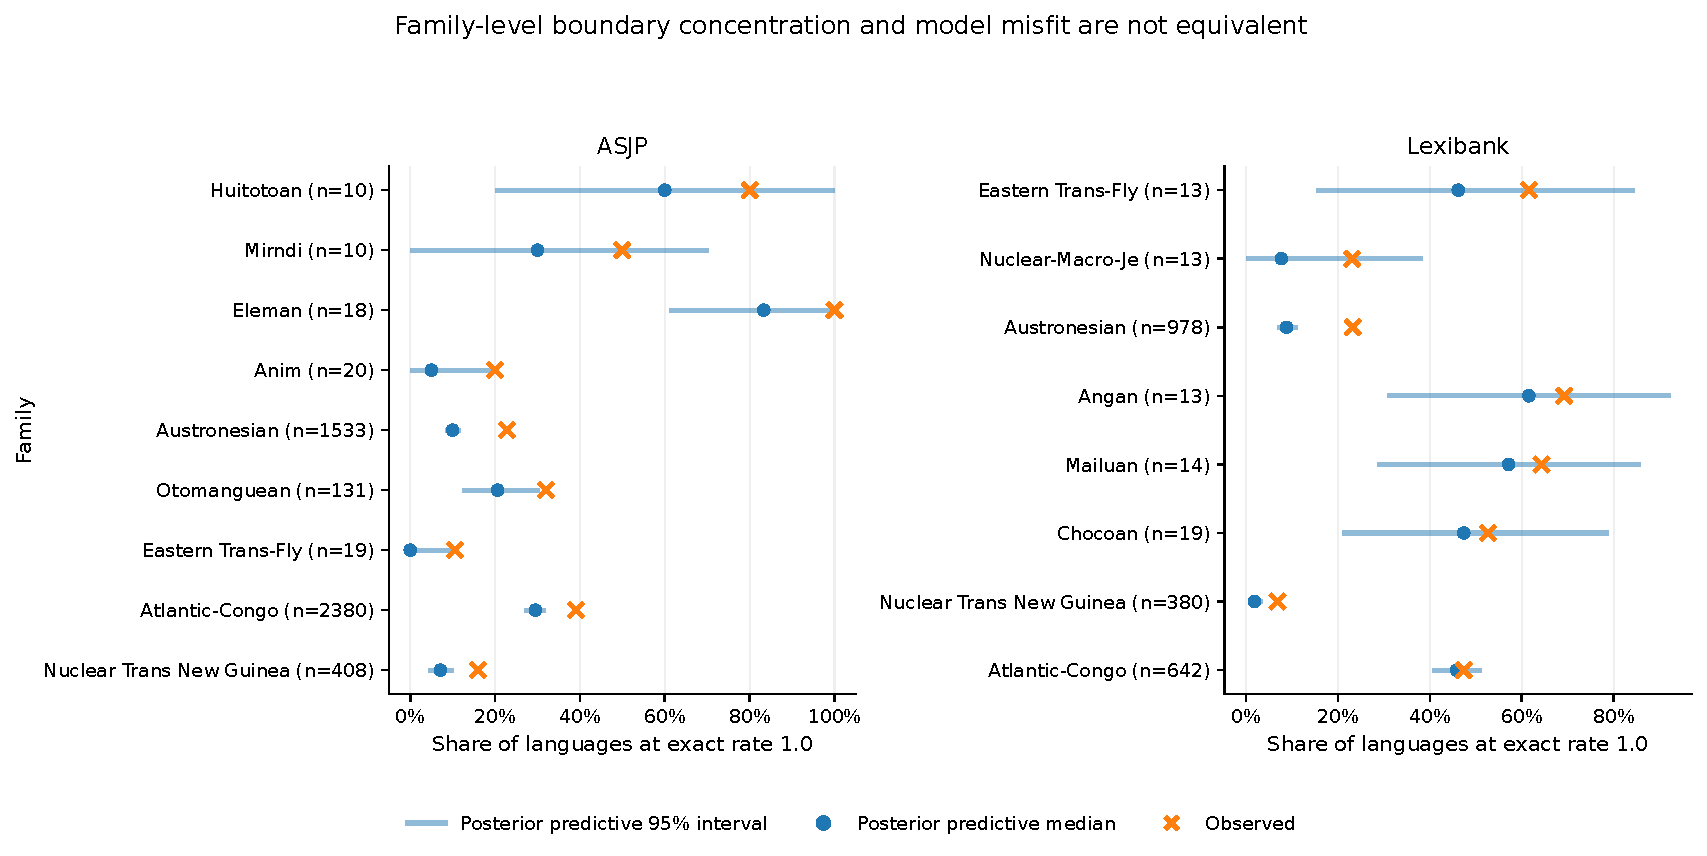
\includegraphics[width=\textwidth]{figures/figureS1_family_boundary_ppc.pdf}
\caption{Family-level boundary concentration and model misfit are not equivalent.
Existing final figure, reused verbatim. Source:
\texttt{results/figureS1\_family\_boundary\_ppc.csv}.}
\label{fig:s1}
\end{figure}
\clearpage

% ============================================================
\section{Areal and hemispheric heterogeneity}
% ============================================================
Broad macroarea adjustment removes approximately 48.0\% of the matched-sample
association (median-based), whereas sample restriction alone produces only a modest
change (Table~\ref{tab:s14}). Macroarea is a broad areal adjustment, not a complete
areal control. The pooled Southern coefficient is not a universal reversal: the
South is regionally heterogeneous (Table~\ref{tab:s15}), and Southern Eurasia
($n=1$) is uninformative and is not interpreted. Latitude must not be treated as a
globally invariant exposure.

\begin{table}[htbp]\centering
\footnotesize
\caption{Matched-sample macroarea adjustment.}
\label{tab:s14}
\resizebox{\ifdim\width>\linewidth \linewidth\else\width\fi}{!}{%
\begin{tabular}{l r r l r r}
\toprule
Model & N lang. & N fam. & $\beta_{\mathrm{lat}}$ [95\% CrI] & OR per SD & Attenuation \\
\midrule
Full primary, family-only & 10,886 & 646 & -0.151 [-0.195, -0.105] & 0.860 & -- \\
Matched, family-only & 10,626 & 386 & -0.138 [-0.183, -0.092] & 0.871 & -- \\
Matched, family + macroarea & 10,626 & 386 & -0.072 [-0.123, -0.021] & 0.931 & 48.0\% \\
\bottomrule
\end{tabular}
}

\par\smallskip{\footnotesize\emph{Note.} Broad macroarea adjustment removes approximately 48.0\% of the matched-sample association (median-based, $1-0.0717/0.1377$). Sample restriction alone (full $\rightarrow$ matched) produces only a modest change. Macroarea is a broad areal adjustment, not a complete areal control; latitude is not a globally invariant exposure.}
\end{table}

\begin{table}[htbp]\centering
\footnotesize
\caption{Southern-Hemisphere macroarea-specific slopes.}
\label{tab:s15}
\resizebox{\ifdim\width>\linewidth \linewidth\else\width\fi}{!}{%
\begin{tabular}{l r r l c c l}
\toprule
Macroarea & N lang. & N fam. & $\beta$ [95\% CrI] & $P(\beta<0)$ & $P(\beta>0)$ & Status \\
\midrule
Papunesia & 2,462 & 124 & 0.545 [0.444, 0.649] & $<$0.001 & $>$0.999 & informative \\
Africa & 952 & 12 & 0.241 [0.114, 0.373] & $<$0.001 & $>$0.999 & informative \\
South America & 354 & 68 & -0.119 [-0.261, 0.021] & 0.951 & 0.049 & informative \\
Australia & 306 & 29 & 0.239 [0.052, 0.429] & 0.006 & 0.994 & informative \\
Eurasia & 1 & 1 & 0.204 [-1.156, 1.580] & 0.390 & 0.610 & uninformative ($n=1$) \\
\bottomrule
\end{tabular}
}

\par\smallskip{\footnotesize\emph{Note.} The pooled Southern coefficient is not a universal reversal: the South is regionally heterogeneous (e.g.\ South America trends negative, Papunesia strongly positive). Southern Eurasia ($n=1$) is uninformative and must not be interpreted.}
\end{table}

\clearpage

% ============================================================
\section{ASJP--Lexibank overlap and comparability}
% ============================================================
ASJP and Lexibank are independently assembled databases with partially overlapping
language coverage; they are not statistically independent language samples. A
descriptive overlap audit would require a stable shared identifier. The committed
Result CSVs contain no shared cross-database identifier (no Glottocode, and no
per-language Lexibank table), and the raw CLDF databases are not part of this
repository, so the overlap cannot be computed from the committed evidence package.
Table~\ref{tab:s16} reports the available counts and marks the non-computable cells
transparently rather than populating them with fabricated values.

\begin{table}[htbp]\centering
\footnotesize
\caption{Cross-database language overlap (audit; not computable from committed artifacts).}
\label{tab:s16}
\resizebox{\ifdim\width>\linewidth \linewidth\else\width\fi}{!}{%
\begin{tabular}{p{0.45\textwidth} r}
\toprule
Quantity & Value \\
\midrule
ASJP primary languages & 10,886 \\
Lexibank languages & 5,501 \\
Shared identifiers & not computable \\
ASJP-only & not computable \\
Lexibank-only & not computable \\
Percentage of ASJP overlapping & not computable \\
Percentage of Lexibank overlapping & not computable \\
Identifier used & none available (no Glottocode / shared key in committed CSVs) \\
Unmatched or ambiguous records & not computable \\
\bottomrule
\end{tabular}
}

\par\smallskip{\footnotesize\emph{Note.} The committed Result CSVs contain no shared cross-database identifier (no Glottocode, and no per-language Lexibank table), and the raw CLDF databases are not in this repository, so the overlap cannot be computed from the committed evidence package. ASJP and Lexibank are independently assembled databases with partially overlapping language coverage; they are not statistically independent language samples. This cell is marked incomplete rather than populated with fabricated values.}
\end{table}

\clearpage

% ============================================================
\section{Computational reproducibility}
% ============================================================
Table~\ref{tab:s17} records the computational environment, distinguishing exact
runtime versions recorded by the notebook from pip installation constraints.
Table~\ref{tab:s18} maps each analysis to its repository and data SHAs, master seed
and offset, Result CSV, NetCDF artifact, figure source, and notebook cell. The
H100/GPU posterior models were not rerun to build this SI.

\begin{table}[htbp]\centering
\footnotesize
\caption{Computational environment.}
\label{tab:s17}
\resizebox{\ifdim\width>\linewidth \linewidth\else\width\fi}{!}{%
\begin{tabular}{l l l l}
\toprule
Component & Recorded runtime version & pip install constraint & Source \\
\midrule
Python & not recorded at runtime & -- & Colab runtime \\
JAX & 0.7.2 & -- & cell 3 stdout \\
NumPyro & 0.19.0 & >=0.16,<0.20 & cell 3 stdout / cell 2 pin \\
ArviZ & not recorded & >=0.20,<0.23 & cell 2 pin \\
pandas & not recorded & >=2.2,<3 & cell 2 pin \\
NumPy & not recorded & -- & bundled with runtime \\
SciPy & not recorded & >=1.13,<2 & cell 2 pin \\
matplotlib & not recorded & >=3.9,<4 & cell 2 pin \\
pyarrow & not recorded & >=17,<22 & cell 2 pin \\
netCDF4 & not recorded & >=1.7 & cell 2 pin \\
Accelerator & CudaDevice(id=0), A100 (declared) & -- & cell 3 / notebook metadata \\
Backend / device & gpu / cuda:0 & -- & reproducibility\_metadata.json \\
\bottomrule
\end{tabular}
}

\par\smallskip{\footnotesize\emph{Note.} pip constraints are installation bounds, not the exact installed versions. Only JAX and NumPyro versions were printed at runtime; Python, ArviZ, pandas, NumPy and SciPy exact versions were not recorded. \texttt{jax\_enable\_x64=True}; master seed 20260711.}
\end{table}

\begin{table}[htbp]\centering
\footnotesize
\caption{Analysis provenance and output-file map.}
\label{tab:s18}
\resizebox{\ifdim\width>\linewidth \linewidth\else\width\fi}{!}{%
\begin{tabular}{l l l l l l l l c}
\toprule
Analysis & Repo SHA & Data SHA & Master seed & Offset & Result CSV & NetCDF artifact & Figure source & Cell \\
\midrule
ASJP BB primary & \texttt{d3ef7a8246} & \texttt{0127953495} & 20260711 & +301 & \texttt{asjp\_beta\_binomial\_primary\_effect.csv} & \texttt{asjp\_beta\_binomial\_primary.nc} & \texttt{figure2\_core\_posterior\_effects.csv} & 72 \\
Lexibank BB replication & \texttt{d3ef7a8246} & \texttt{edf5f028de} & 20260711 & +305 & \texttt{lexibank\_beta\_binomial\_replication\_effect.csv} & \texttt{lexibank\_beta\_binomial\_replication.nc} & \texttt{figure2\_core\_posterior\_effects.csv} & 80 \\
ASJP BB within/between & \texttt{d3ef7a8246} & \texttt{0127953495} & 20260711 & +302 & \texttt{asjp\_beta\_binomial\_within\_between\_effects.csv} & \texttt{asjp\_beta\_binomial\_within\_between.nc} & \texttt{figure2\_core\_posterior\_effects.csv} & 74 \\
ASJP BB positional & \texttt{d3ef7a8246} & \texttt{0127953495} & 20260711 & +303 & \texttt{asjp\_beta\_binomial\_position\_effects.csv} & \texttt{asjp\_beta\_binomial\_position\_interaction.nc} & \texttt{figure1\_position\_specific\_gradients.csv} & 76 \\
ASJP BB hemisphere & \texttt{d3ef7a8246} & \texttt{0127953495} & 20260711 & +304 & \texttt{asjp\_beta\_binomial\_hemisphere\_effects.csv} & \texttt{asjp\_beta\_binomial\_hemisphere.nc} & \texttt{figure2\_core\_posterior\_effects.csv} & 78 \\
ASJP BB family+macroarea & \texttt{d3ef7a8246} & \texttt{0127953495} & 20260711 & +306 & \texttt{asjp\_beta\_binomial\_macroarea\_effect.csv} & \texttt{asjp\_beta\_binomial\_macroarea\_control.nc} & \texttt{figure3\_macroarea\_attenuation.csv} & 85 \\
ASJP BB Southern macroarea & \texttt{d3ef7a8246} & \texttt{0127953495} & 20260711 & +307 & \texttt{asjp\_beta\_binomial\_south\_macroarea\_effects.csv} & \texttt{asjp\_beta\_binomial\_south\_macroarea\_slopes.nc} & \texttt{figure3\_southern\_macroarea\_slopes.csv} & 86 \\
ASJP BB matched, no macroarea & \texttt{d3ef7a8246} & \texttt{0127953495} & 20260711 & +308 & \texttt{asjp\_beta\_binomial\_macroarea\_matched\_comparison.csv} & \texttt{asjp\_beta\_binomial\_macroarea\_matched\_no\_macroarea.nc} & \texttt{figure3\_macroarea\_attenuation.csv} & 100 \\
Leave-family-out & \texttt{d3ef7a8246} & \texttt{0127953495} & 20260711 & +410 & \texttt{asjp\_boundary\_family\_exclusion\_sensitivity.csv} & \texttt{(not committed)} & \texttt{figure2\_core\_posterior\_effects.csv} & 95 \\
Leave-top-two positional & \texttt{d3ef7a8246} & \texttt{0127953495} & 20260711 & +420 & \texttt{asjp\_position\_excluding\_top\_two\_boundary\_families.csv} & \texttt{(not committed)} & \texttt{figure2\_core\_posterior\_effects.csv} & 97 \\
\bottomrule
\end{tabular}
}

\par\smallskip{\footnotesize\emph{Note.} Repo SHA is the results-provenance SHA from \texttt{reproducibility\_metadata.json}; the SI was built at HEAD \texttt{562dee88b5}. NetCDF posterior artifacts are named by the notebook but are not committed to the repository; the H100/GPU models were NOT rerun to build this SI.}
\end{table}

\clearpage

\section*{Data and code availability}
All tables and figures in this SI are generated from the Result CSV files in
\texttt{results/} by the scripts in \texttt{supplement/scripts/}. Provenance and
publication-facing values are recorded in \texttt{supplement/manifest.json}; the
per-cell notebook inventory, source ledger, claim-to-evidence map, manuscript
contract, and validation/consistency reports are in \texttt{supplement/generated/}.
Data sources: ASJP \citep{asjp2022}, Lexibank \citep{list2022lexibank}, Glottolog
\citep{glottolog2023}. Inference used NumPyro \citep{phan2019numpyro} on JAX
\citep{jax2018} with ArviZ \citep{kumar2019arviz} diagnostics.

\bibliographystyle{elsarticle-num}
\bibliography{supplement}

\end{document}
